% !TEX TS-program = pdflatex
% !TEX encoding = UTF-8 Unicode

% This is a simple template for a LaTeX document using the "article" class.
% See "book", "report", "letter" for other types of document.

\documentclass[11pt]{report} % use larger type; default would be 10pt

\usepackage[utf8]{inputenc} % set input encoding (not needed with XeLaTeX)

%%% Examples of Article customizations
% These packages are optional, depending whether you want the features they provide.
% See the LaTeX Companion or other references for full information.

%%% PAGE DIMENSIONS

\usepackage[a4paper,left=2.5cm,right=2.5cm,top=2.5cm,bottom=2.5cm]{geometry}
%\usepackage{geometry} % to change the page dimensions
%\geometry{a4paper} % or letterpaper (US) or a5paper or....
% \geometry{margin=2in} % for example, change the margins to 2 inches all round
% \geometry{landscape} % set up the page for landscape
%   read geometry.pdf for detailed page layout information

\usepackage{graphicx} % support the \includegraphics command and options

% \usepackage[parfill]{parskip} % Activate to begin paragraphs with an empty line rather than an indent

%%% PACKAGES
\usepackage{booktabs} % for much better looking tables
\usepackage{array} % for better arrays (eg matrices) in maths
\usepackage{paralist} % very flexible & customisable lists (eg. enumerate/itemize, etc.)
\usepackage{verbatim} % adds environment for commenting out blocks of text & for better verbatim
\usepackage{subfig} % make it possible to include more than one captioned figure/table in a single float
% These packages are all incorporated in the memoir class to one degree or another...

%%% HEADERS & FOOTERS
\usepackage{fancyhdr} % This should be set AFTER setting up the page geometry
\pagestyle{fancy} % options: empty , plain , fancy
\renewcommand{\headrulewidth}{0pt} % customise the layout...
\lhead{}\chead{}\rhead{}
\lfoot{}\cfoot{\thepage}\rfoot{}

%%% SECTION TITLE APPEARANCE
\usepackage{sectsty}
\allsectionsfont{\sffamily\mdseries\upshape} % (See the fntguide.pdf for font help)
% (This matches ConTeXt defaults)

%%% ToC (table of contents) APPEARANCE
\usepackage[nottoc,notlof,notlot]{tocbibind} % Put the bibliography in the ToC
\usepackage[titles,subfigure]{tocloft} % Alter the style of the Table of Contents
\renewcommand{\cftsecfont}{\rmfamily\mdseries\upshape}
\renewcommand{\cftsecpagefont}{\rmfamily\mdseries\upshape} % No bold!

% Default fixed font does not support bold face
\DeclareFixedFont{\ttb}{T1}{txtt}{bx}{n}{12} % for bold
\DeclareFixedFont{\ttm}{T1}{txtt}{m}{n}{12}  % for normal

% Custom colors
\usepackage{color}
\definecolor{deepblue}{rgb}{0,0,0.5}
\definecolor{deepred}{rgb}{0.6,0,0}
\definecolor{deepgreen}{rgb}{0,0.5,0}

\usepackage{listings}

% Python style for highlighting
\newcommand\pythonstyle{\lstset{
language=Python,
basicstyle=\ttm,
otherkeywords={self},             % Add keywords here
keywordstyle=\ttb\color{deepblue},
emph={MyClass,__init__},          % Custom highlighting
emphstyle=\ttb\color{deepred},    % Custom highlighting style
stringstyle=\color{deepgreen},
frame=tb,                         % Any extra options here
showstringspaces=false            % 
}}


% Python environment
\lstnewenvironment{python}[1][]
{
\pythonstyle
\lstset{#1}
}
{}

% Python for external files
\newcommand\pythonexternal[2][]{{
\pythonstyle
\lstinputlisting[#1]{#2}}}

% Python for inline
\newcommand\pythoninline[1]{{\pythonstyle\lstinline!#1!}}

% hyper reference
\usepackage{hyperref}

%%% END Article customizations

%%% The "real" document content comes below...

\title{Basic Information on 23-ID-1}
\author{Wenjie Chen}
%\date{} % Activate to display a given date or no date (if empty),
         % otherwise the current date is printed 

\begin{document}
\maketitle

\section{Introduction}

This is a brief report on NSLS-II CSX beamline 23-ID-1, Brookhaven National Laboratory. I came here to do research on $\rm ZrTe_3$ from Nov. 15th to Nov. 22th in 2017. 

There was a slideshow of introduction to this beamline written by Professor Li before, but when I came on site, some commands have been changed to meet a higher standard of Python programming style. On the other hand, some explanations in the old slideshow seemed unclear to me (e.g., the layout), so I think it might be better to write a new document. Therefore, here it comes. 

If you have any questions, please feel free to contact me.\footnote{E-mail: wenjiechen@pku.edu.cn}

\section{The Diffractometer}
\subsection{Layout}
There are three angles very important for the diffractometer. Together, they formed the geometry we required for the measurement.
\begin{center}
\begin{tabular}{|c|c|}\hline
angles & Descriptions\\ \hline
$\delta$ & The angle between the detector and the horizontal plane.\\ \hline
$\theta$ & The angle between the sample plane and the horizontal plane. \\ \hline
$\gamma$ & The angle between the detector and the $yz$ plane. \\ \hline
\end{tabular}
\end{center}

The coordinate system is shown in Fig.\ref{fig:layout}, along with the angles mentioned above.
\begin{figure}[h!]
\centering
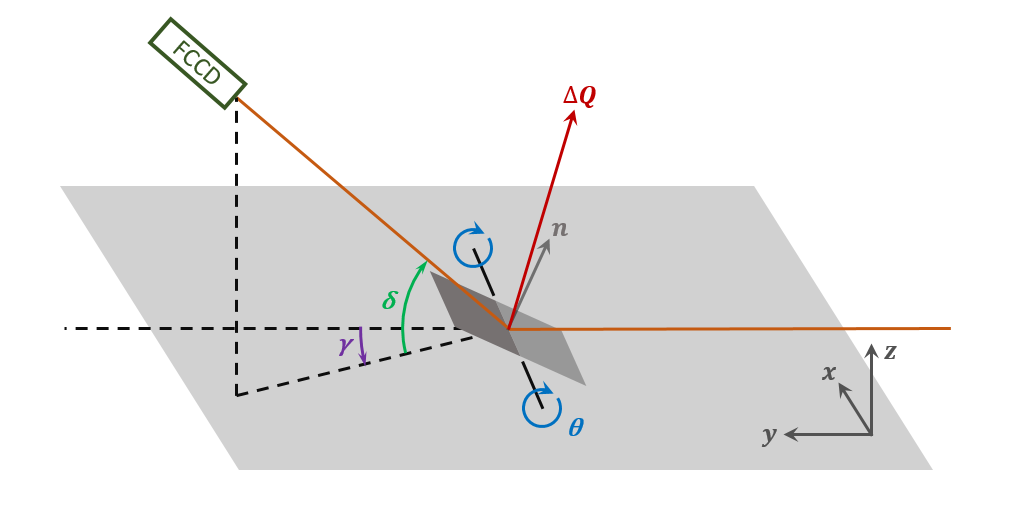
\includegraphics[width=140mm]{layout.PNG}
\caption{\label{fig:layout}%
The diffractometer's layout.}
\end{figure}

\subsection{Control and Movements}
All movements are driven by motors. We can change both the angles and the position of the sample. 

One thing you should keep in mind is that some commands make \textbf{relative} movements (relative to current angles or position), while others make \textbf{absolute} movements.

To change these angles, either type in GUI panels, or use the following commands in IPython:
\begin{python}
tardis.position 
    '''return the current reciprocal position of tardis'''
tardis.real_position 
    '''return the current real position of tardis'''
tardis.forward(h, k, l)
    '''return the angles for observing (h, k, l) signal'''
tardis.move(h, k, l) 
    '''move the tardis to receive (h, k, l) signal'''
\end{python}

To change the position of the sample, either type in GUI panels, or use the following commands in IPython:
\begin{python}
RE(mv(sx, v1, sy, v2, sz, v3))
    '''move the sample to (x, y, z) = (v1, v2, v3)'''
\end{python}

\subsection{Scan}
According to \textbf{Bluesky}'s specification, all movements are done with ``Run Engine''. (Go to the last section for more information about \textbf{Bluesky}.) Therefore, basically every commands about movements will look like this:
\begin{python}
RE(mv(variable1, value1, variable2, value2, ...))
\end{python}
Here the variables and values are not necessarily to have simple data structures. Instead, the variables are always defined to be some class, and the values are either float numbers or lists/tuples. The assignments are automatically treated by the \pythoninline{mv(*args)} function.

\section{Frequently Used Terms}
In this section, several frequently used terms will be introduced in details.
\begin{center}
\begin{tabular}{|c|c|}\hline
Terms & Descriptions\\ \hline
tardis & The synchrotron diffractometer used here.\\ \hline

\end{tabular}
\end{center}

\section{Frequently Used Functions}
In this section, several frequently used Python functions will be introduced in details.

\begin{center}
\begin{tabular}{|c|c|}\hline
Terms & Descriptions\\ \hline
RE & abbr. for Run Engine. Used when operating hardware through codes. \\ \hline

\end{tabular}
\end{center}

\section{``In-text'' listing highlighting}

\begin{python}
class MyClass(Yourclass):
    def __init__(self, my, yours):
        bla = '5 1 2 3 4'
        print bla
\end{python}

\section{External listing highlighting}

%\pythonexternal{demo.py}

\section{Inline highlighting}

Definition \pythoninline{class MyClass} means \dots

\section{More Information}
NSLS-II has an organization on GitHub (\url{https://github.com/NSLS-II}). I recommend viewing it and saving it to your bookmarks.

The documentation on \textbf{bluesky} is also very useful (\url{http://nsls-ii.github.io/bluesky/}). Bluesky is a library for experiment control and collection of scientific data and metadata. There you can learn about how NSLS-II works with more details.

\end{document}
